\chapter{Experiments}
\label{cha:experiments}
\vspace{0.4 cm}

In this chapter, we're going to delve into the experiments we've crafted to put our approach into action and assess its performance. We describe the design, implementation, and evaluation steps, providing a detailed account of each experiment. These experiments are crucial to demonstrating the effectiveness and practicality of our approach in real-world scenarios.

\section{Preprocessing}
\label{sec:exp_preprocessing}
\vspace{0.2 cm}
Within this sub-chapter, we will elaborate on our methodology for assembling a collection of Java projects. We outline the procedures involved in generating test cases using EvoSuite and Randoop\cite{noauthor_randoop_nodate}, shedding light on the steps taken to ensure comprehensive test coverage. Additionally, we will discuss the process of preparing corresponding focal methods, elucidating how we identify and associate the specific methods targeted by each test case. This step is crucial in establishing a robust foundation for subsequent analyses and evaluations within the realm of software testing and development.

\vspace{0.1 cm}
\subsection{Java Projects Selection}
\label{sec:projects_selection}
\vspace{0.1 cm}

We carefully selected four projects, as outlined in Table \ref{tab:collected_java_projects}, from the pool of publicly available GitHub Java repositories that declare an open-source license. Our selection criteria also considered popularity, with priority given to projects boasting the highest number of stars or forks. Emphasizing diversity, we aimed to cover a spectrum of project types. Here are the project selection criteria that we followed:\\
    \begin{enumerate}
        \item \textbf{Preventing Data Leakage:} To mitigate the risk of unintentional data exposure, we systematically exclude potential repositories that might be part of the pretraining data for the considered LLMs. Our focus lies on projects updated within the past three years to ensure relevance.
        
        \item \textbf{Maven Compatibility:} To streamline subsequent processes, we narrow down our dataset to repositories utilizing Maven as the package manager. This decision is based on the presence of a pom.xml file at the repository root, indicating Maven usage.

        \item \textbf{Class Threshold:} We eliminate repositories with fewer than 40 classes to avoid selecting overly simplistic projects that might not offer substantial complexity.
        
        \item \textbf{Compilation Check:} Ensuring the compilability of repositories is crucial. We mandate that all dependencies be specified in the pom.xml files and selected Java version (Java 1.8). The compilation process is executed with the command 
        \begin{verbatim}
        mvn clean compile
        \end{verbatim} and repositories failing to compile are excluded. Although roughly half of the repositories compile successfully, further exploration of compilation errors might enhance compilation success rates in future endeavors.
        
        \item \textbf{Execution Check:} Similar to the compilation criterion, we require repositories to be executable in our environment. Following the selection of the Java version, we execute the command 
        \begin{verbatim}
        cd target
        java -jar <PROJECT-SNAPSHOT>.jar
        \end{verbatim}
        and retain repositories where the command succeeds. Logs are saved for future reference, and potential investigation into reasons for execution failures is left for future work.
    \end{enumerate}
From these chosen projects, encompassing a total of 388 classes, we further refined our sample by randomly selecting nine classes, totaling 87 methods. This selection process ensures that our tool encounters a diverse range of scenarios and project structures, contributing to a more comprehensive evaluation. Further details about these chosen classes can be found in Table \ref{tab:selected_java_projects}.

\begin{table}[htbp]
    \centering
    \begin{tabular}{l | l | r}
        \textbf{Project Name} & \textbf{Classes} & \textbf{Reference} \\
        \hline
        frontend-maven-plugin & 43 & \cite{sletteberg_frontend-maven-plugin_2023} \\
        javacv & 117 & \cite{noauthor_bytedecojavacv_nodate} \\
        webdrivermanager & 44 & \cite{noauthor_bonigarciawebdrivermanager_nodate} \\
        zerocode & 184 & \cite{noauthor_authorjappszerocode_nodate} \\
    \end{tabular}
\caption{Details of the collected Java projects.}
\label{tab:collected_java_projects}
\end{table}

\begin{table}
    \centering    
    \begin{tabular}{l | l | r}
        \textbf{Class Name} & \textbf{Project Name} & \textbf{Methods} \\
        \hline
        BaseSettings & javacv & 6 \\
        Parallel & javacv & 6 \\
        SeekableByteArrayOutputStream & javacv & 3 \\
        NPMInstaller & frontend-maven-plugin & 15 \\
        NodeInstaller & frontend-maven-plugin & 18 \\
        PnpmInstaller & frontend-maven-plugin & 14 \\
        CacheHandler & webdrivermanager & 4 \\
        PropertiesProviderUtils & zerocode & 4 \\
        ZerocodeCorrelationshipLogger & zerocode & 17 \\
    \end{tabular}
\caption{Details of the classes from the selected Java projects.}
\label{tab:selected_java_projects}
\end{table}

\vspace{0.1 cm}
\subsection{Test Case Generation with EvoSuite}
\label{sec:test_case_generation}
\vspace{0.1 cm}

For our experiments, we utilized EvoSuite to generate automated test cases for each of the selected classes. We adhered to the default configurations of EvoSuite, setting the search budget to 15 and opting not to minimize. We generated 9 Test Suites with a total of 138 test cases. The generated test suites for each class are outlined in Table \ref{tab:evosuite_testclasses}.

\begin{table}
    \centering    
    \begin{tabular}{l | l | r}
        \textbf{Test Suite} & \textbf{Class Name} & \textbf{Test Cases} \\
        \hline
        BaseSettings\_ESTest & BaseSettings & 14 \\
        Parallel\_ESTest & Parallel & 6 \\
        SeekableByteArrayOutputStream\_ESTest & SeekableByteArrayOutputStream & 13 \\
        NPMInstaller\_ESTest & NPMInstaller & 18 \\
        NodeInstaller\_ESTest & NodeInstaller & 18 \\
        PnpmInstaller\_ESTest & PnpmInstaller & 21 \\
        CacheHandler\_ESTest & CacheHandler & 13 \\
        PropertiesProviderUtils\_ESTest & PropertiesProviderUtils & 14 \\
        ZerocodeCorrelationshipLogger\_ESTest & ZerocodeCorrelationshipLogger & 21 \\
    \end{tabular}
\caption{Summary of EvoSuite generated test classes.}
\label{tab:evosuite_testclasses}
\end{table}
    
\vspace{0.1 cm}
\subsection{LLM Selection and Configuration}
\label{sec:llm_configurations}
\vspace{0.1 cm}

Our tool offers flexibility in LLM selection, allowing developers to choose models based on their preferences. To seamlessly integrate a specific LLM into our framework, developers need to load the corresponding configurations for that particular model. For our experiments, we opted for models acknowledged for their performance, relying on the HuggingFace\cite{noauthor_hugging_2023} Open LLM Leaderboard\cite{open-llm-leaderboard} as a reference. We carefully selected five top-performing models, as highlighted in Table~\ref{tab:selected_models}, presenting the LLM benchmark.

This approach empowers users to tailor their LLM choices, ensuring compatibility and aligning with their project requirements. The decision to incorporate well-regarded models from the leaderboard enhances the credibility and effectiveness of our experiments.

\begin{table}[htbp]
    \centering    
    \begin{tabular}{l | c | c | c | c | c | r}
        \textbf{Model} & \textbf{Average} & \textbf{ARC} & \textbf{HellaSwag} & \textbf{MMLU} & \textbf{TruthfulQA} & \textbf{Reference} \\
        \hline
        \scriptsize\textsc{mpt-7b-chat} & 49.95 & 46.5 & 75.51 & 37.62 & 40.16 & \cite{MosaicML2023Introducing}\cite{noauthor_mosaicmlmpt-7b-chat_2023}  \\
        \scriptsize\textsc{Nous-Hermes-13b} & 60.15 & 56.57 & 82.11 & 50.44 & 51.5 & \cite{noauthor_nousresearchnous-hermes-13b_nodate} \\
        \scriptsize\textsc{orca\_mini\_v3\_13b}  & \textbf{63.45*} & \textbf{63.14*} & \textbf{82.35*} & \textbf{56.52*} & 51.81 & \cite{noauthor_pankajmathurorca_mini_v3_13b_2023}\cite{mukherjee2023orca}\\
        \scriptsize\textsc{stable-vicuna-13B}  & 57.63 & 53.33 & 78.5 & 50.29 & 48.38 & \cite{noauthor_theblokestable-vicuna-13b-hf_2023} \\
        \scriptsize\textsc{WizardLM-13B-V1.1}  & 60.55 & 58.62 & 81.07 & 48.32 & \textbf{54.19*} & \cite{noauthor_theblokewizardlm-13b-v1-1-superhot-8k-fp16_nodate}\cite{vicuna2023} \\
    \end{tabular}
\caption{OpenLLM Leaderboard Benchmarks for Selected Models}
\label{tab:selected_models}
\end{table}

In the preliminary phase of our experimentation, we conducted local trials with various configurations to fine-tune the settings for our Large Language Models (LLMs). These configurations play a pivotal role in shaping the characteristics of our tool, EvoOracle, which focuses on test oracle generation. Based on the results obtained from our local experiments and considering the significance of each configuration parameter, we opted for a set of parameters that strike a delicate balance between precision, diversity, and computational efficiency. With a low temperature of 0.1, our chosen configuration ensures deterministic and focused predictions. Simultaneously, the generous n\_predict value of 4096 allows for a broad spectrum of predictions, promoting diversity. Setting top-p to 0.95 and top-k to 40 emphasizes the consideration of high-probability tokens during sampling. The chosen batch size of 9 optimizes computational resources. Lastly, the repeat penalty and repeat last N parameters, both set at 1.1, encourage non-repetitive and varied output. This meticulous selection of configurations from our local trials serves as a foundation for the subsequent large-scale experiments on the cluster, ensuring an optimal balance between assertive precision and computational efficiency.

\vspace{0.1 cm}
\subsection{Prompt Preparation and Assertion Generation}
\label{sec:prompt_preparation}
\vspace{0.1 cm}

Before settling on our final approach for effective assertion generation, we conducted a series of preliminary experiments. The goal was to refine our prompt strategy, ensuring that it aligns optimally with the intricacies of the code context. After careful consideration and evaluation, we arrived at a well-crafted prompt, which is detailed in Listing~\ref{prompt_template}. This strategic decision to leverage a specific prompt stems from the insights gained through experimentation, aiming to enhance the clarity and relevance of instructions provided to the Large Language Models (LLMs). Our iterative process of refining prompts has been instrumental in shaping an approach that maximizes the LLMs' understanding of code contexts and subsequently improves the precision of assertion generation.

\begin{lstlisting}[style=llm_prompt, label=prompt_template, caption=Prompt Template]
### Instruction:
You are working with a Java project which includes a class called 
`{{ class_name }}` and has some methods.
Method details as JSON: `{{ method_details }}`.
You are tasked with generating a test oracle for a JUnit test case 
based on the above information of the method to test its functionality .
### Prompt:
In the following the test case, replace the `{{ assertion_placeholder }}` 
with one or more appropriate assertions:
```
{{ test_method_code }}
```
Write the assertion statement using following pattern:
```r'(\w+\.)?(assert|assertTrue|assertNull|fail|assertFalse|assertNotEquals
|assertEquals|assertArrayEquals|assertNotNull|assertNotSame|assertSame
|assertThat)\s*\(.+?\);'```
Assertion must end with ```;```

### Response:
\end{lstlisting}

\section{Experimental Setup}
\label{sec:experimental_setup}
\vspace{0.2 cm}

For our experimental setup, we conducted the experiments on a dedicated High-Performance Computing (HPC) cluster equipped with four nodes. Each node features Intel Xeon CPU 6226R\cite{noauthor_intel_nodate} processors running at 2.9GHz, with a configuration of 32 CPUs and 16GB of RAM. To ensure consistency and reproducibility, we created a specialized Singularity\cite{noauthor_introduction_nodate} image version v3.8.7\cite{noauthor_singularity_releases_nodate} with Java 1.8 and Python 3.10 and all the Python required libraries~\ref{} tailored for our implemented tool, enabling seamless execution on the HPC cluster. This configuration allowed us to leverage the cluster's computational capabilities effectively for our experimentation.

We conducted a total of 9660 experiments, exploring various configurations of test cases, models, oracle types, and repetitions. The distribution of experiments is outlined by the following equation:
\[
N_e = TC \times M \times OT \times R = 138 \times 5 \times 2 \times 7 = 9660
\]
Here, \\
N\textsubscript{e} = Number of experiments\\
TC = Test Cases\\
M = Models\\
OT = Oracle Type\\
R = Repetitions\\
After the generation of oracles and completion of the execution process, we conduct an evaluation by scrutinizing various output files and logs. This analysis encompasses examination of build logs, test execution outputs, and coverage files.
\noindent
We conducted experiments by considering two variants of Oracle type, 
\begin{enumerate}
    \item \textbf{Test cases with EvoOracle assertions:} We only use the Oracles generated by EvoOracle.
    \item \textbf{Test cases with EvoSuite + EvoOracle assertions:} We keep the EvoSuite Oracles and complement them by adding EvoOracle assertions to them.
\end{enumerate}
\vspace{0.1 cm}
\subsection{Evaluation Metrics}
\label{sec:evaluation_metrics}
\vspace{0.1 cm}
After the generation of oracles and completion of the execution process, we conduct an evaluation by analyzing various output files and logs. This analysis encompasses examination of build logs, test execution outputs, and coverage files. We consider several quantitative measures used to assess and evaluate different aspects of our experimental results. These metrics provide a systematic and standardized way to gauge the performance, efficiency, and effectiveness of our proposed approach. They serve as numerical indicators that help us draw meaningful conclusions about the capabilities and limitations of our solution in the realm of automated test oracle generation using Large Language Models.

    \begin{enumerate}
        \item \textbf{Coverage Metrics:}
        \begin{itemize}
            \item \textbf{Line Coverage:} This metric measures the proportion of lines of code that are executed by the test suite. It gives an overview of how much of the code is exercised during testing. The formula for calculating line coverage \(LC\) is given by:
\[
LC = \frac{\text{{Number of Covered Lines}}}{\text{{Total Number of Lines}}}
\]

            \item \textbf{Mutation Coverage:} This metric measures and analyzes after introducing mutations into the code how many of these mutations are detected by the test suite. Mutation coverage reflects the ability of tests to identify and handle different types of faults.
            The formula for mutation coverage ($\mu$\textsubscript{c}) is given by:
\[
\mu_{\text{c}} = \frac{\text{{killed mutants}}}{\text{{total mutants}}}
\]
            \item \textbf{Test Strength:} This is a metric that considers both line coverage and mutation coverage. It provides a holistic view of how well the tests exercise the code and how effective they are at detecting mutations. The formula for calculating test strength \(\tau\textsubscript{s}\) is given by:
\[
\tau_{\text{s}} = \frac{\text{{killed mutants}}}{\text{{covered mutants}}}
\]
        \end{itemize}
    \end{enumerate}

    In addition to coverage, we present four additional metrics to quantify the number of test cases at specific stages of the pipeline:

    \begin{enumerate}
        \item \textbf{Syntax Correctness:} Number of tests that do not have syntax errors. Meaning, the count of test cases adhering to the Java grammar.
        \item \textbf{Compilable:} The tests count that have correct syntax and do not fail during build. Count of test cases that successfully compiled in their scaffolding without errors, measured both absolutely and relative to the Unique count.
        \item \textbf{Failing Test:} The test builds successfully but fails due to wrong assertions or expected behavior.
        \item \textbf{Passing Test:} The test builds and passes successfully;
        \item \textbf{Correct:} Count of test cases that were compiled and executed without errors and invoked the correct Method Under Test (MUT), measured both absolutely and relative to the Unique count. 
    \end{enumerate}
    This metric is adopted from Tufano et al. \cite{tufano_unit_2021} which provides comparability across different repositories.

\section{Research Questions}
\label{sec:research_questions}
\vspace{0.2 cm}

In this section, we will discuss the research questions. We set out to answer with our experiments:
\begin{itemize}
    \item \textbf{RQ1: How is the quality of the EvoOracle generated Oracles?}\\
    In examining the quality of EvoOracle-generated Oracles, we assess the following metrics:
    \begin{itemize}
        \item Syntax Correctness
        \item Compilable
        \item Failing Test
        \item Passing Test
        \item Correct
    \end{itemize}
    In addition to quantitative metrics, qualitative examination involves manual analysis of correct and failing tests. Through this comprehensive evaluation, we aim to provide a nuanced understanding of the EvoOracle-generated Oracles' quality, combining quantitative rigor with qualitative insights.
    
    \item \textbf{RQ2: How does the performance of EvoOracle generated assertions compare to assertions generated by traditional automated test generation tool, EvoSuite?}\\
    To assess the comparative performance, we employ mutation testing on the test suites generated by both EvoOracle and EvoSuite. We use mutation coverage, test strength and line coverage to evaluate the performance of both tool.
    
    \item \textbf{RQ3: How does the performance of EvoSuite change if they are complemented with EvoOracle generated assertions?}\\
    Instead of replacing the asserions in EvoSuite, we enhance the them by adding the EvoOracle generated assertions to them. Then we run mutation testing again to see how the EvoOracle enahance EvoSuite tests compare against the individual EvoSuite and EvoOracle.
    
    \item \textbf{RQ4: How many attempts are typically needed for successful assertion generation, and does the success rate improve with additional attempts following initial failure?}\\
    This research question aims to understand the efficiency of assertion generation by quantifying the number of attempts required for success. The measurement involves tracking the count of attempts made for assertion generation during the experimental process. To answer this question, we analyze the success and failure instances, categorizing them based on the number of attempts made. By examining the patterns of successful assertion generation over multiple attempts, we gain insights into the effectiveness of iterative prompting and identify whether additional attempts contribute to increased success rates. This exploration helps evaluate the practicality and reliability of the assertion generation process, guiding developers on optimal strategies when dealing with failed attempts.
    
    \item \textbf{RQ5: How well-suited is the proposed LLM-based assertion generation approach for practical integration into real-world software development workflows, and what challenges and practical considerations arise from its implementation?}\\
    We analyze the time consumed by the tool to generate assertions.
    % \item \textbf{RQ5:} Context size, dependency thing, How many methods were fed for prompt?
    % \textbf{MAKE IT BETTER.}
    
    % \item \textbf{RQ6:} To what extent can LLMs generalize across different software projects and programming paradigms when generating test assertions?
\end{itemize}

\section{Results}
\label{sec:results}
\vspace{0.2 cm}

In this section, we discuss the results for ... 

\vspace{0.1 cm}
\subsection{RQ1}
\label{sec:results_rq1}
\vspace{0.1 cm}

In this subsection, an overview of ...

\begin{table}[H]
\centering

\begin{tabular}{| l | r | r | r | r | r | r |}
\hline
\multirow{2}{*}{\textbf{Class}} & \multirow{2}{*}{\textbf{EvoSuite}} & \multicolumn{5}{c|}{\textbf{EvoOracle}} \\ % Fix multicolumn formatting
\cline{3-7} % Add a horizontal line between the headers
 &  & \textbf{MPT-7B} & \textbf{Nous} & \textbf{Orca} & \textbf{Stable} & \textbf{WizardLM} \\
 &  &  & \textbf{hermes-13b} & \textbf{mini\_13B} & \textbf{Vicuna-13B} & \textbf{13B-V1.1} \\
\hline
\scriptsize\textsc{} &  &  &  &  &  &  \\
\scriptsize\textsc{BaseSettings} & \textbf{53.33\%} & 34.29\% & 42.86\% & 32.29\% & 48.43\% & 26.60\% \\
\hline
\scriptsize\textsc{} &  &  &  &  &  &  \\
\scriptsize\textsc{CacheHandler} & \textbf{27.78\%} & 0.00\% & 1.57\% & 0.00\% & 0.00\% & 0.00\% \\
\hline
\scriptsize\textsc{} &  &  &  &  &  &  \\
\scriptsize\textsc{NPMInstaller} & \textbf{34.09\%} & 3.29\% & 15.00\% & 0.00\% & 0.00\% & 0.00\% \\
\hline
\scriptsize\textsc{} &  &  &  &  &  &  \\
\scriptsize\textsc{NodeInstaller} & \textbf{56.9\%} & 39.60\% & 45.14\% & 23.33\% & 0.00\% & 5.14\% \\
\hline
\scriptsize\textsc{} &  &  &  &  &  &  \\
\scriptsize\textsc{Parallel} & \textbf{100\%} & 26.00\% & 50.57\% & 31.00\% & 31.57\% & 52.86\% \\
\hline
\scriptsize\textsc{} &  &  &  &  &  &  \\
\scriptsize\textsc{PnpmInstaller} & \textbf{29.27\%} & 13.00\% & 17.00\% & 0.00\% & 2.14\% & 5.50\% \\
\hline
\scriptsize\textsc{Properties} &  &  &  &  &  &  \\
\scriptsize\textsc{ProviderUtils} & \textbf{26.67\%} & 16.43\% & 12.57\% & 12.57\% & 19.00\% & 13.43\% \\
\hline
\scriptsize\textsc{SeekableByte} &  &  &  &  &  &  \\
\scriptsize\textsc{ArrayOutputStream} & \textbf{93.75\%} & 1.50\% & 57.29\% & 22.00\% & 31.00\% & 19.83\% \\
\hline
\scriptsize\textsc{Zerocode} &  &  &  &  &  &  \\
\scriptsize\textsc{Correlationship} &  &  &  &  &  &  \\
\scriptsize\textsc{Logger} & \textbf{52.38\%} & 17.67\% & 28.71\% & 19.33\% & 27.57\% & 28.86\% \\
\hline

\end{tabular}
\caption{Average Mutation Coverage by Class and Models.\protect\footnotemark}
\label{tab:mutation_coverage}
\end{table}
\footnotetext{Significant values are highlighted with bold fonts.}

\begin{table}[H]
\centering

\begin{tabular}{| l | r | r | r | r | r | r |}
\hline
\multirow{2}{*}{\textbf{Class}} & \multirow{2}{*}{\textbf{EvoSuite}} & \multicolumn{5}{c|}{\textbf{EvoSuite + EvoOracle}} \\ % Fix multicolumn formatting
\cline{3-7} % Add a horizontal line between the headers
 &  & \textbf{MPT-7B} & \textbf{Nous} & \textbf{Orca} & \textbf{Stable} & \textbf{WizardLM} \\
 &  &  & \textbf{hermes-13b} & \textbf{mini\_13B} & \textbf{Vicuna-13B} & \textbf{13B-V1.1} \\
\hline
\scriptsize\textsc{} &  &  &  &  &  &  \\
\scriptsize\textsc{BaseSettings} & \textbf{53.33\%} & 52.38\% & 47.62\% & 38.09\% & 52.38\% & 31.43\% \\
\hline
\scriptsize\textsc{} &  &  &  &  &  &  \\
\scriptsize\textsc{CacheHandler} & \textbf{27.78\%} & 26.99\% & 23.02\% & 15.87\% & \textbf{27.78\%} & \textbf{27.78\%}  \\
\hline
\scriptsize\textsc{} &  &  &  &  &  &  \\
\scriptsize\textsc{NPMInstaller} & \textbf{34.09\%} & 32.79\% & 31.50\% & 4.92\% & \textbf{34.09\%} & 25.97\%  \\
\hline
\scriptsize\textsc{} &  &  &  &  &  &  \\
\scriptsize\textsc{NodeInstaller} & \textbf{56.9\%} & 55.66\% & 50.49\% & 42.61\% & \textbf{56.90\%} & 6.65\%  \\
\hline
\scriptsize\textsc{} &  &  &  &  &  &  \\
\scriptsize\textsc{Parallel} & \textbf{100\%} & 52.75\% & 55.50\% & 30.77\% & 54.95\% & 56.60\%  \\
\hline
\scriptsize\textsc{} &  &  &  &  &  &  \\
\scriptsize\textsc{PnpmInstaller} & \textbf{29.27\%} & \textbf{29.27\%} & \textbf{29.27\%} & 2.09\% & \textbf{29.27\%} & 16.37\%  \\
\hline
\scriptsize\textsc{Properties} &  &  &  &  &  &  \\
\scriptsize\textsc{ProviderUtils} & \textbf{26.67\%} & \textbf{26.67\%} & \textbf{26.67\%} & 22.86\% & \textbf{26.67\%} & \textbf{26.67\%}  \\
\hline
\scriptsize\textsc{SeekableByte} &  &  &  &  &  &  \\
\scriptsize\textsc{ArrayOutputStream} & \textbf{93.75\%} & 89.29\% & 91.96\% & 25.00\% & \textbf{93.75\%} & 41.96\%  \\
\hline
\scriptsize\textsc{Zerocode} &  &  &  &  &  &  \\
\scriptsize\textsc{Correlationship} &  &  &  &  &  &  \\
\scriptsize\textsc{Logger} & \textbf{52.38\%} & 48.30\% & 49.66\% & 35.37\% & \textbf{52.38\%} & 51.70\%  \\
\hline

\end{tabular}
\caption{Average Mutation Coverage by Class and Models for EvoSuite tests enhanced with EvoOracle assetions.\protect\footnotemark}
\label{tab:mutation_coverage}
\end{table}

\footnotetext{Significant values are highlighted with bold fonts.}
\begin{table}[H]
\centering

\begin{tabular}{| l | r | r | r | r | r | r |}
\hline
\multirow{2}{*}{\textbf{Class}} & \multirow{2}{*}{\textbf{EvoSuite}} & \multicolumn{5}{c|}{\textbf{EvoOracle}} \\ % Fix multicolumn formatting
\cline{3-7} % Add a horizontal line between the headers
 &  & \textbf{MPT-7B} & \textbf{Nous} & \textbf{Orca} & \textbf{Stable} & \textbf{WizardLM} \\
 &  &  & \textbf{hermes-13b} & \textbf{mini\_13B} & \textbf{Vicuna-13B} & \textbf{13B-V1.1} \\
\hline
\scriptsize\textsc{} &  &  &  &  &  &  \\
\scriptsize\textsc{BaseSettings} & \textbf{53.33\%} & 36.14\% & 43.29\% & 33.86\% & 48.43\% & 26.60\% \\
\hline
\scriptsize\textsc{} &  &  &  &  &  &  \\
\scriptsize\textsc{CacheHandler} & \textbf{71.43\%} & 0.00\% & 5.71\% & 0.00\% & 0.00\% & 0.00\% \\
\hline
\scriptsize\textsc{} &  &  &  &  &  &  \\
\scriptsize\textsc{NPMInstaller} & 71.43\% & 93.71\% & 85.67\% & \textbf{100\%} & \textbf{100\%} & \textbf{100\%} \\
\hline
\scriptsize\textsc{} &  &  &  &  &  &  \\
\scriptsize\textsc{NodeInstaller} & \textbf{100\%} & 91.60\% & 98.29\% & 69.00\% & 0.00\% & 98.71\% \\
\hline
\scriptsize\textsc{} &  &  &  &  &  &  \\
\scriptsize\textsc{Parallel} & \textbf{100\%} & 29.00\% & 52.86\% & 31.00\% & 33.43\% & 54.86\% \\
\hline
\scriptsize\textsc{} &  &  &  &  &  &  \\
\scriptsize\textsc{PnpmInstaller} & 70.59\% & 55.29\% & 54.33\% & 57.14\% & \textbf{100\%} & 48.75\% \\
\hline
\scriptsize\textsc{Properties} &  &  &  &  &  &  \\
\scriptsize\textsc{ProviderUtils} & \textbf{66.67\%} & 45.43\% & 40.29\% & 40.29\% & 47.57\% & 34.57\% \\
\hline
\scriptsize\textsc{SeekableByte} &  &  &  &  &  &  \\
\scriptsize\textsc{ArrayOutputStream} & 93.75\% & 5.00\% & 64.29\% & 66.50\% & \textbf{100\%} & 37.83\% \\
\hline
\scriptsize\textsc{Zerocode} &  &  &  &  &  &  \\
\scriptsize\textsc{Correlationship} &  &  &  &  &  &  \\
\scriptsize\textsc{Logger} & \textbf{55\%} & 25.33\% & 33.29\% & 44.83\% & 34.29\% & 41.43\% \\
\hline

\end{tabular}
\caption{Average Test Strength by Class and Models.\protect\footnotemark}
\label{tab:test_strength}
\end{table}

\begin{table}[H]
\centering

\begin{tabular}{| l | r | r | r | r | r | r |}
\hline
\multirow{2}{*}{\textbf{Class}} & \multirow{2}{*}{\textbf{EvoSuite}} & \multicolumn{5}{c|}{\textbf{EvoOracle}} \\ % Fix multicolumn formatting
\cline{3-7} % Add a horizontal line between the headers
 &  & \textbf{MPT-7B} & \textbf{Nous} & \textbf{Orca} & \textbf{Stable} & \textbf{WizardLM} \\
 &  &  & \textbf{hermes-13b} & \textbf{mini\_13B} & \textbf{Vicuna-13B} & \textbf{13B-V1.1} \\
\hline
\scriptsize\textsc{} &  &  &  &  &  &  \\
\scriptsize\textsc{BaseSettings} & \textbf{100\%} & 92.71 & 98.86 & 92.71 & 99.43 & 64.40 \\
\hline
\scriptsize\textsc{} &  &  &  &  &  &  \\
\scriptsize\textsc{CacheHandler} & \textbf{51.52\%} & 0.00 & 43.71 & 39.60 & 0.00 & 36.00 \\
\hline
\scriptsize\textsc{} &  &  &  &  &  &  \\
\scriptsize\textsc{NPMInstaller} & \textbf{46.49\%} & 10.71 & 23.67 & 6.00 & 6.00 & 6.00 \\
\hline
\scriptsize\textsc{} &  &  &  &  &  &  \\
\scriptsize\textsc{NodeInstaller} & \textbf{53.04\%} & 38.20 & 40.43 & 26.00 & 0.00 & 5.86 \\
\hline
\scriptsize\textsc{} &  &  &  &  &  &  \\
\scriptsize\textsc{Parallel} & \textbf{100\%} & 69.25 & 90.29 & 98.00 & 83.00 & 91.71 \\
\hline
\scriptsize\textsc{} &  &  &  &  &  &  \\
\scriptsize\textsc{PnpmInstaller} & \textbf{41.53\%} & 25.43 & 34.67 & 7.43 & 4.43 & 17.25 \\
\hline
\scriptsize\textsc{Properties} &  &  &  &  &  &  \\
\scriptsize\textsc{ProviderUtils} & \textbf{57.14\%} & 45.00 & 45.00 & 38.71 & 57.00 & 53.00 \\
\hline
\scriptsize\textsc{SeekableByte} &  &  &  &  &  &  \\
\scriptsize\textsc{ArrayOutputStream} & \textbf{100\%} & 36.25 & 77.57 & 28.00 & 31.00 & 47.00 \\
\hline
\scriptsize\textsc{Zerocode} &  &  &  &  &  &  \\
\scriptsize\textsc{Correlationship} &  &  &  &  &  &  \\
\scriptsize\textsc{Logger} & \textbf{91.38\%} & 74.00 & 86.71 & 53.00 & 85.57 & 72.00 \\
\hline

\end{tabular}
\caption{Average Line Coverage by Class and Models.\protect\footnotemark}
\label{tab:line_coverage}
\end{table}
\footnotetext{Significant values are highlighted with bold fonts.}

\begin{figure}[H]
\centering
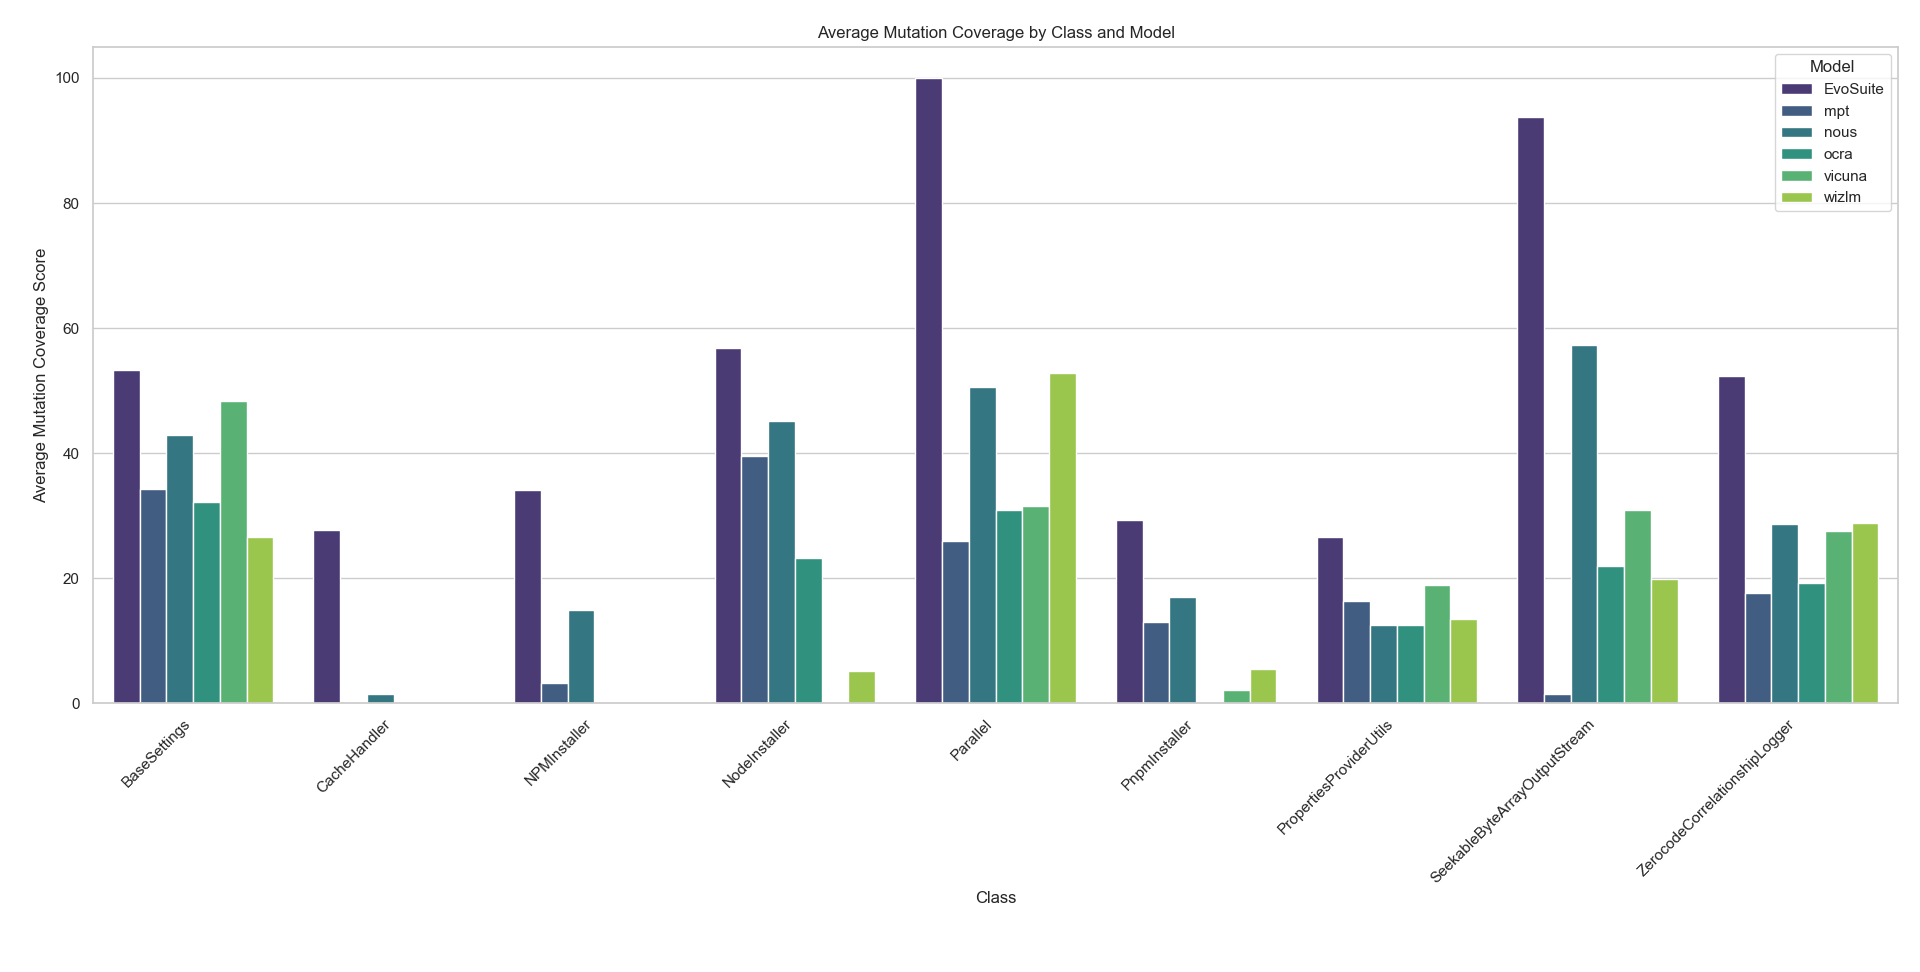
\includegraphics[width=1\textwidth]{images/mutation_coverage_avg.png}
\caption{Average Mutation Coverage by Class and Models}
\label{fig:mutation_coverage}
\end{figure}

\begin{figure}[H]
\centering
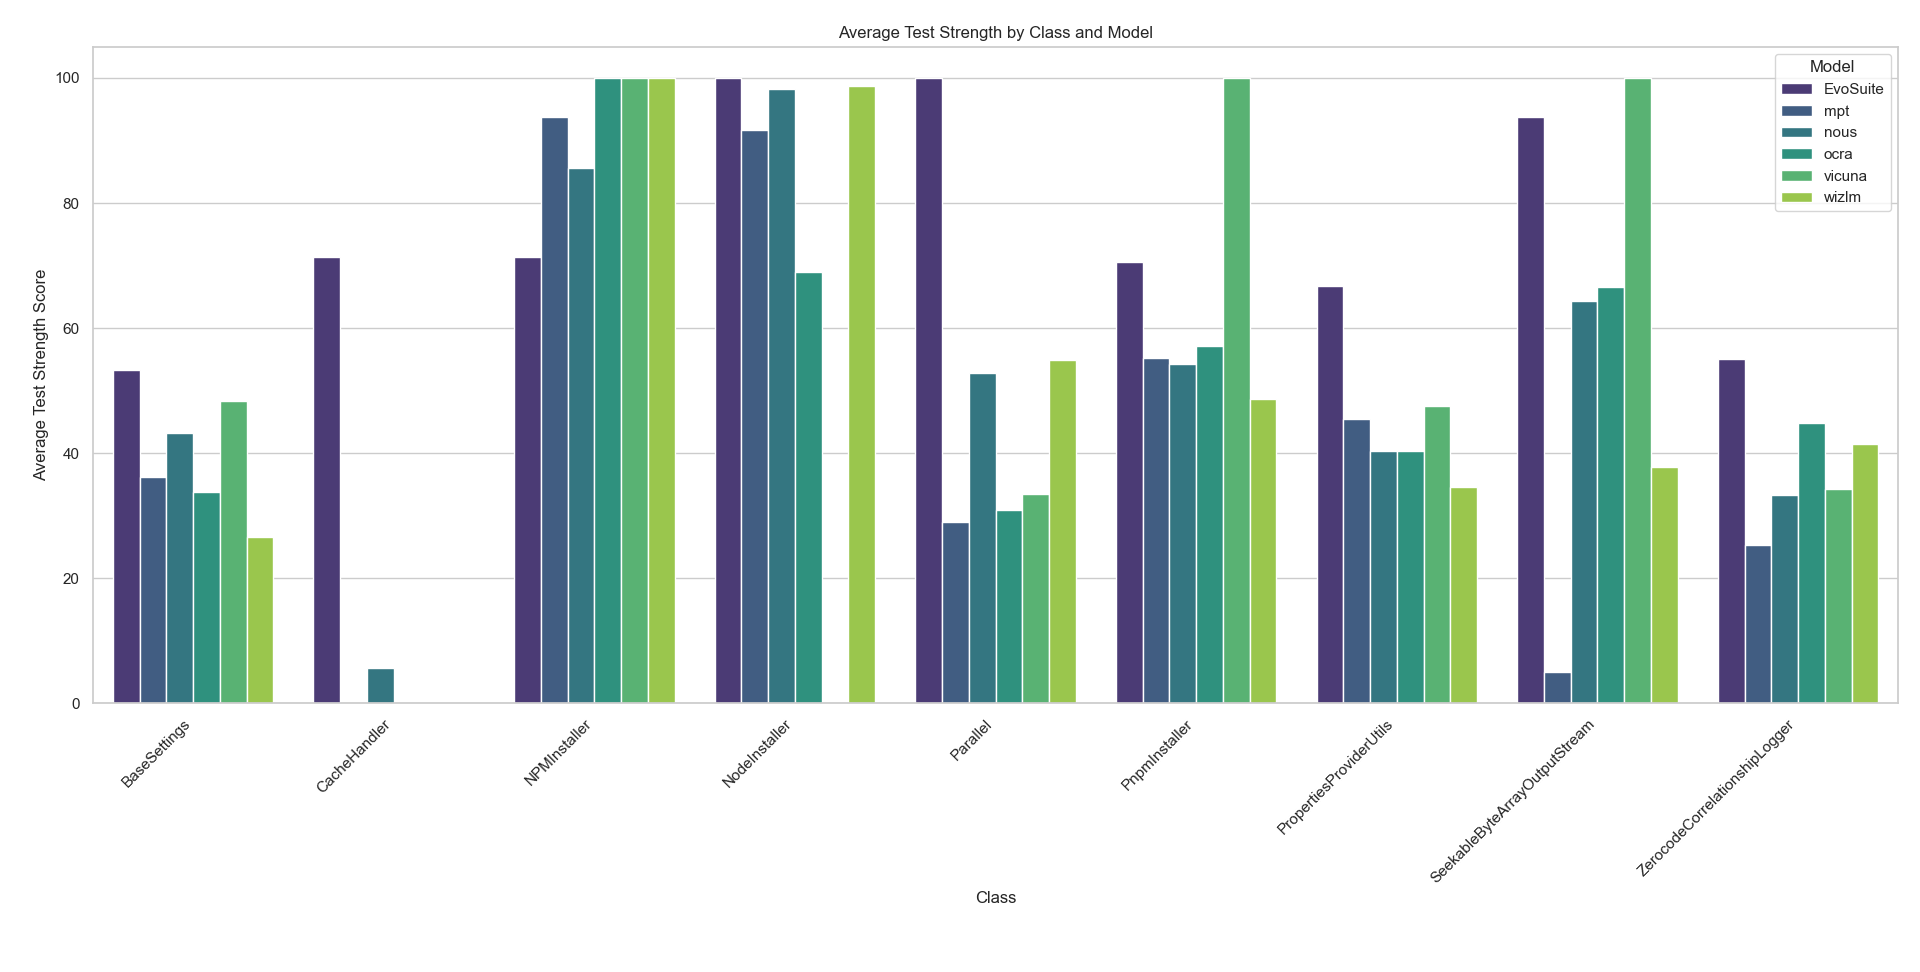
\includegraphics[width=1\textwidth]{images/test_strength_avg.png}
\caption{Average Test Strength by Class and Models}
\label{fig:test_strength}
\end{figure}

\begin{figure}[H]
\centering
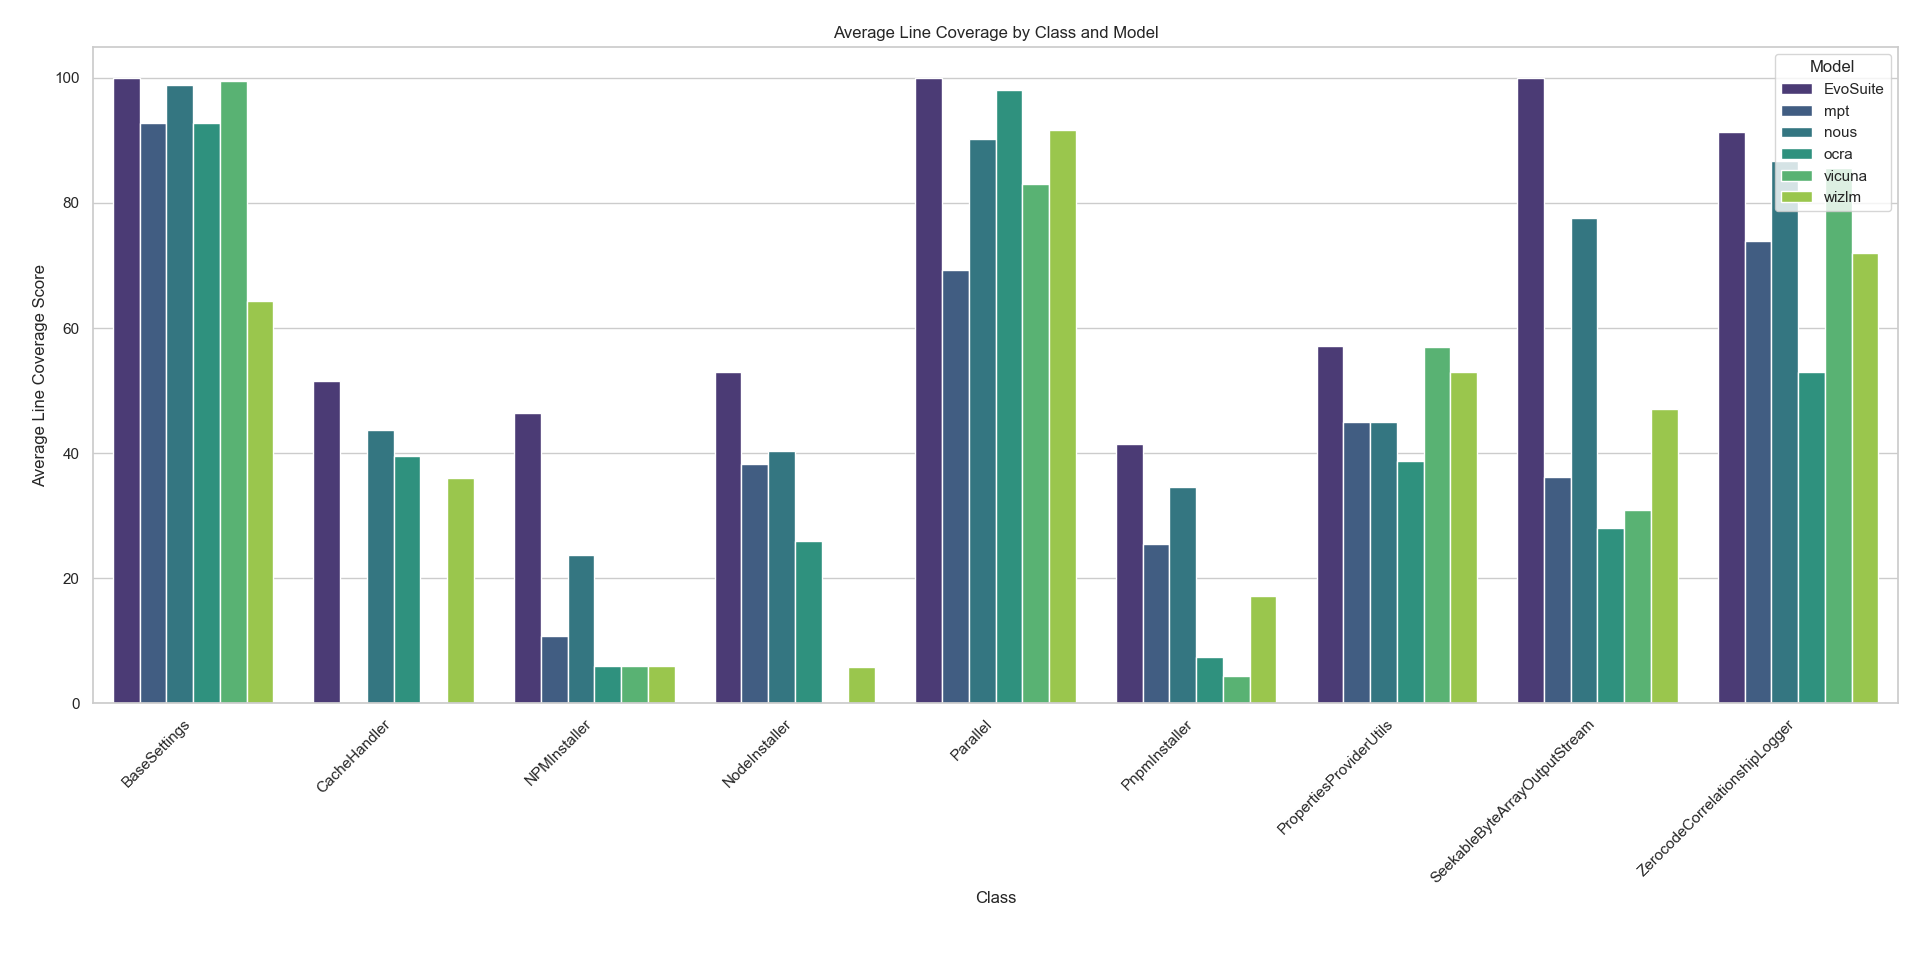
\includegraphics[width=1\textwidth]{images/line_coverage_avg.png}
\caption{Average Line Coverage by Class and Models}
\label{fig:line_coverage}
\end{figure}

\begin{figure}[H]
\centering
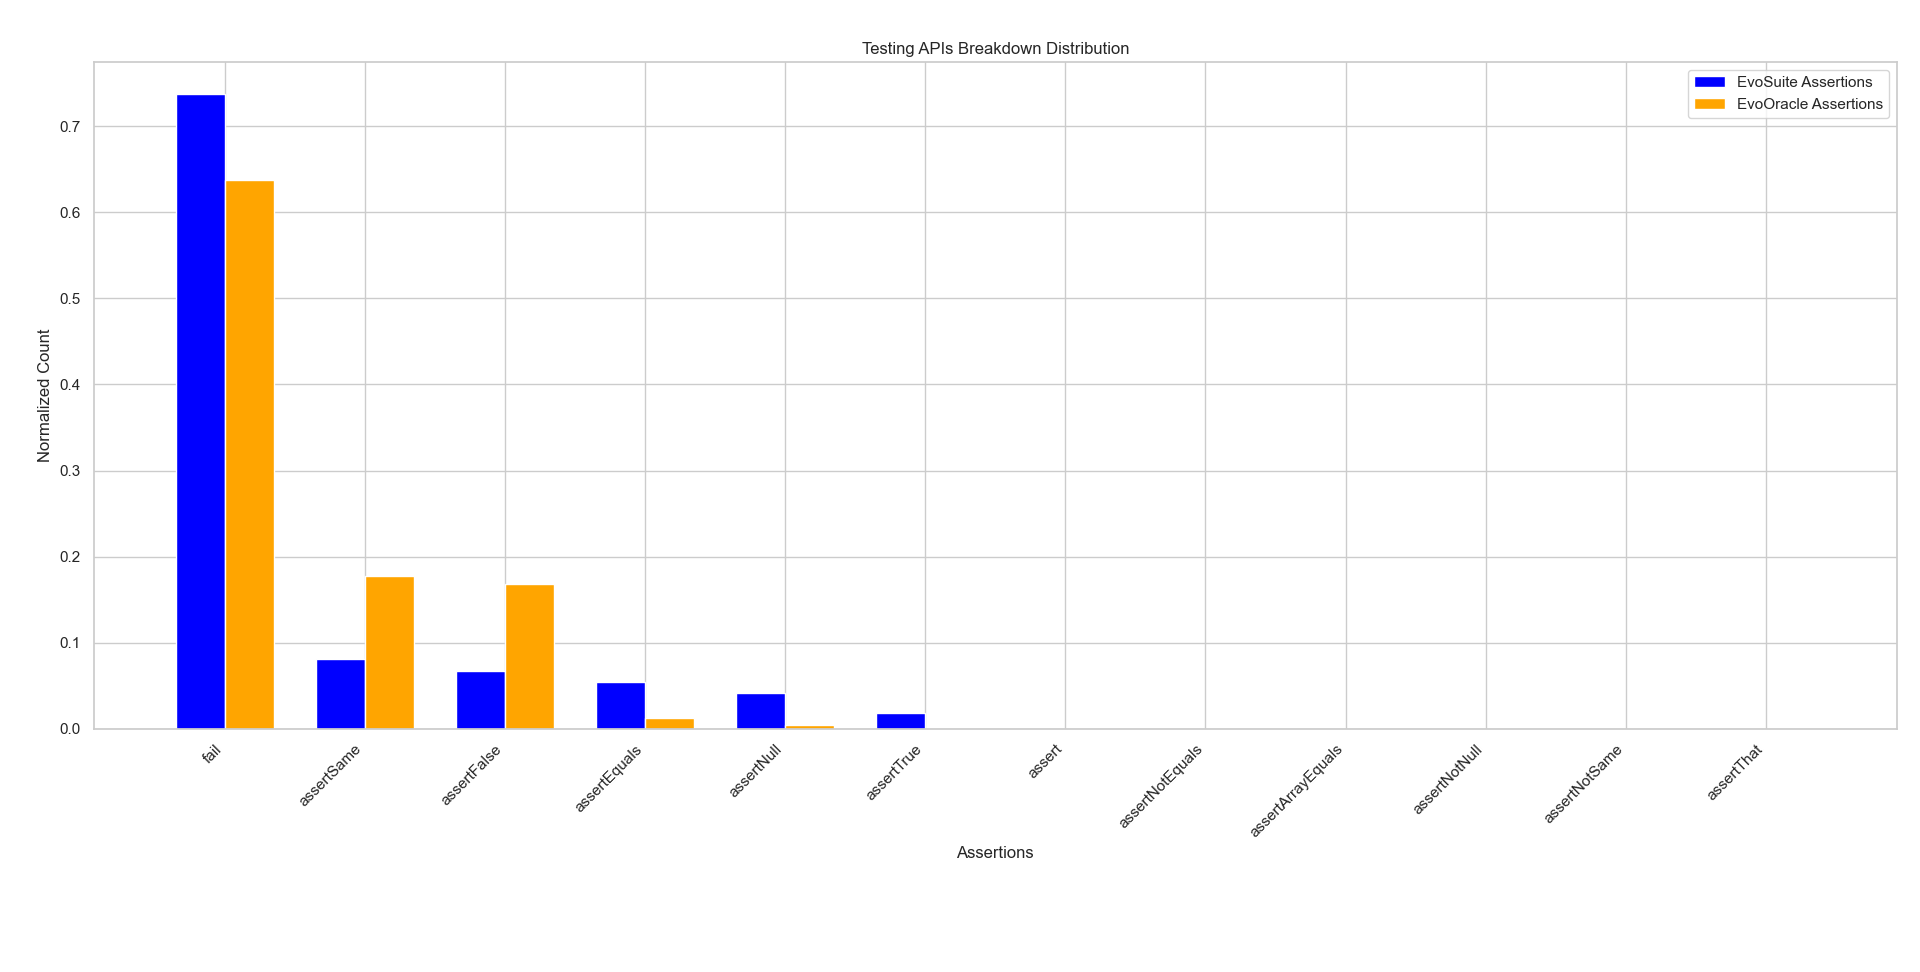
\includegraphics[width=1\textwidth]{images/test_api_distribution.png}
\caption{Testing APIs Breakdown Distribution: EvoSuite vs EvoOracle}
\label{fig:test_api_distribution}
\end{figure}

\begin{figure}[H]
\centering
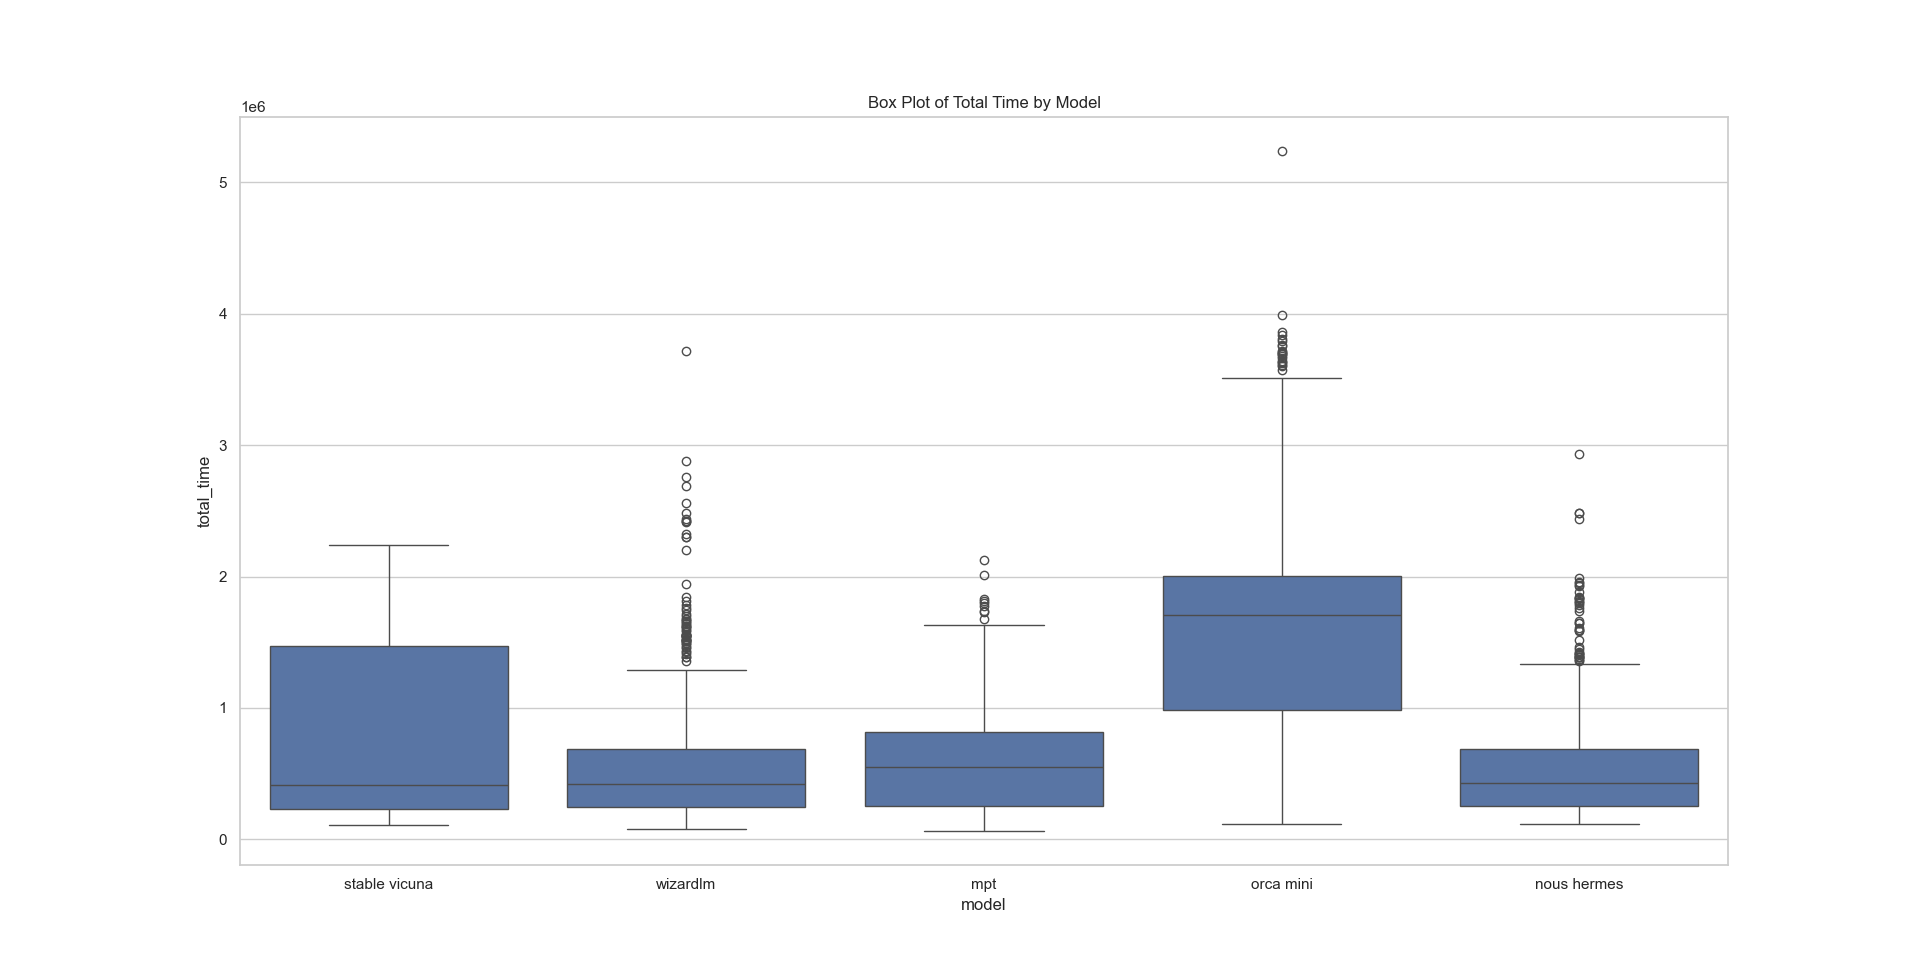
\includegraphics[width=1\textwidth]{images/time_by_model.png}
\caption{Total time taken by Models}
\label{fig:time_models}
\end{figure}

\begin{figure}[H]
\centering
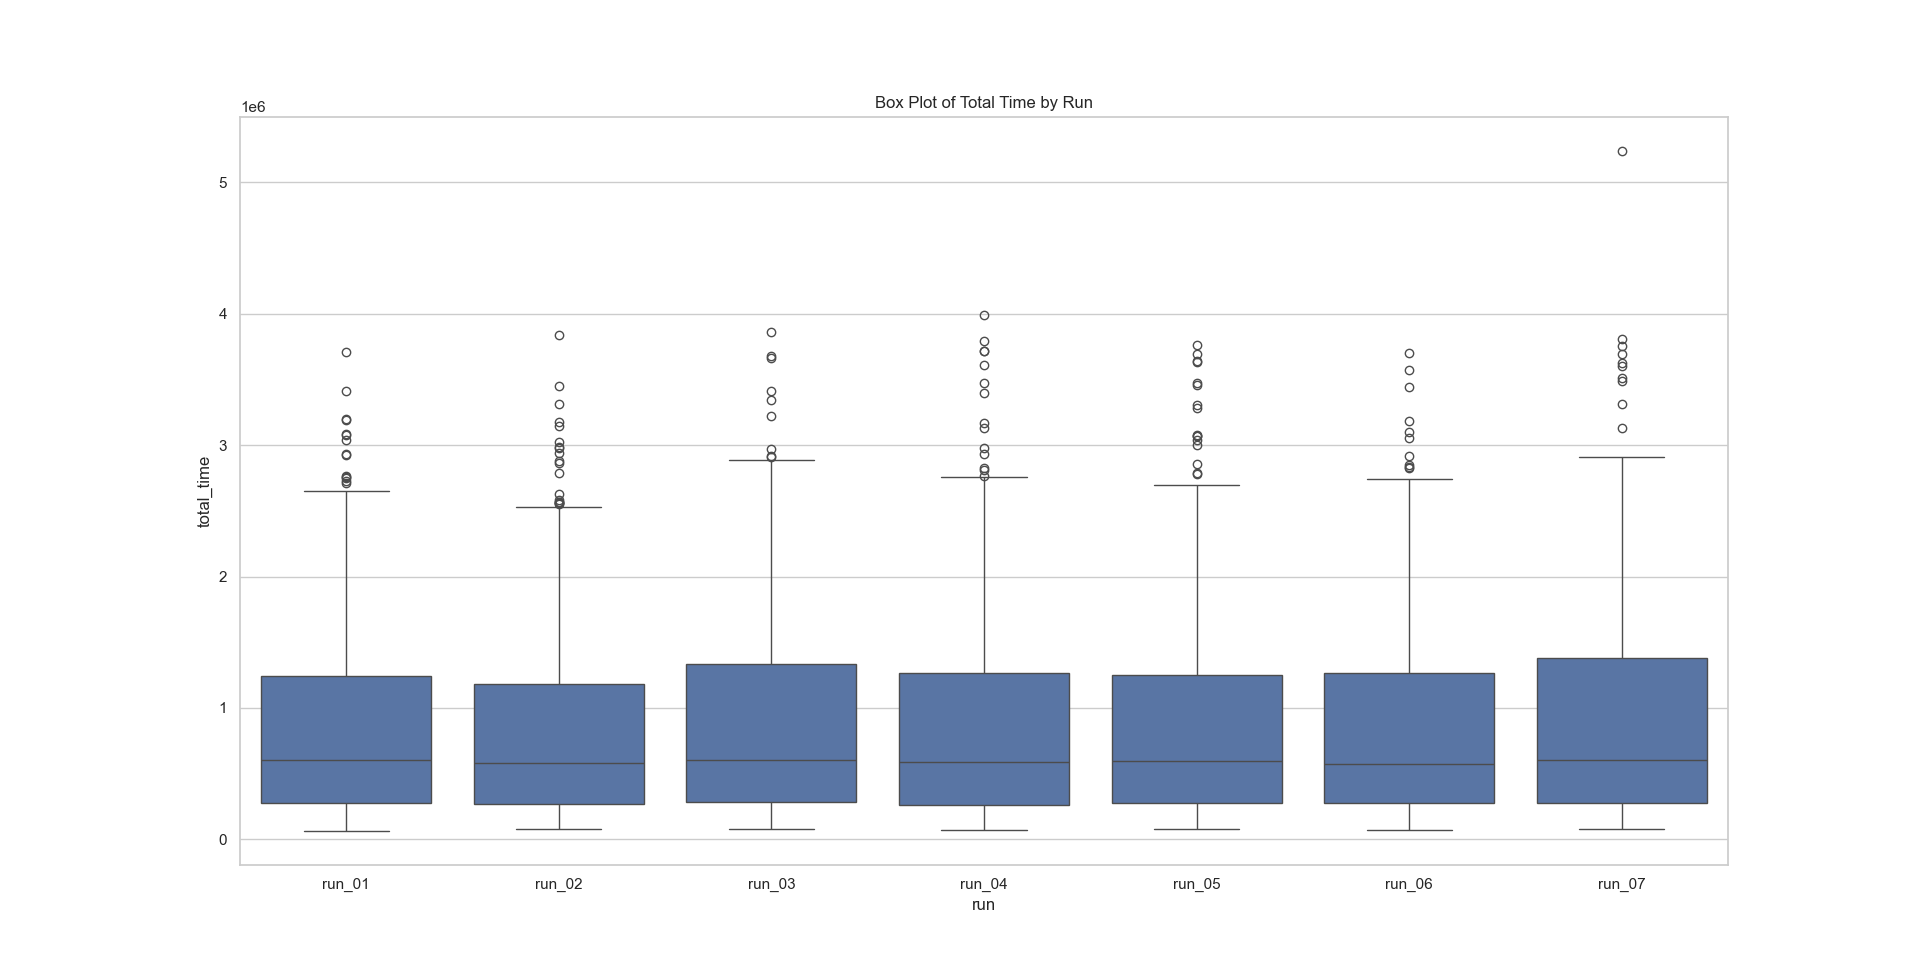
\includegraphics[width=1\textwidth]{images/time_by_runs.png}
\caption{Total time taken by each run}
\label{fig:time_runs}
\end{figure}

\begin{figure}[H]
\centering
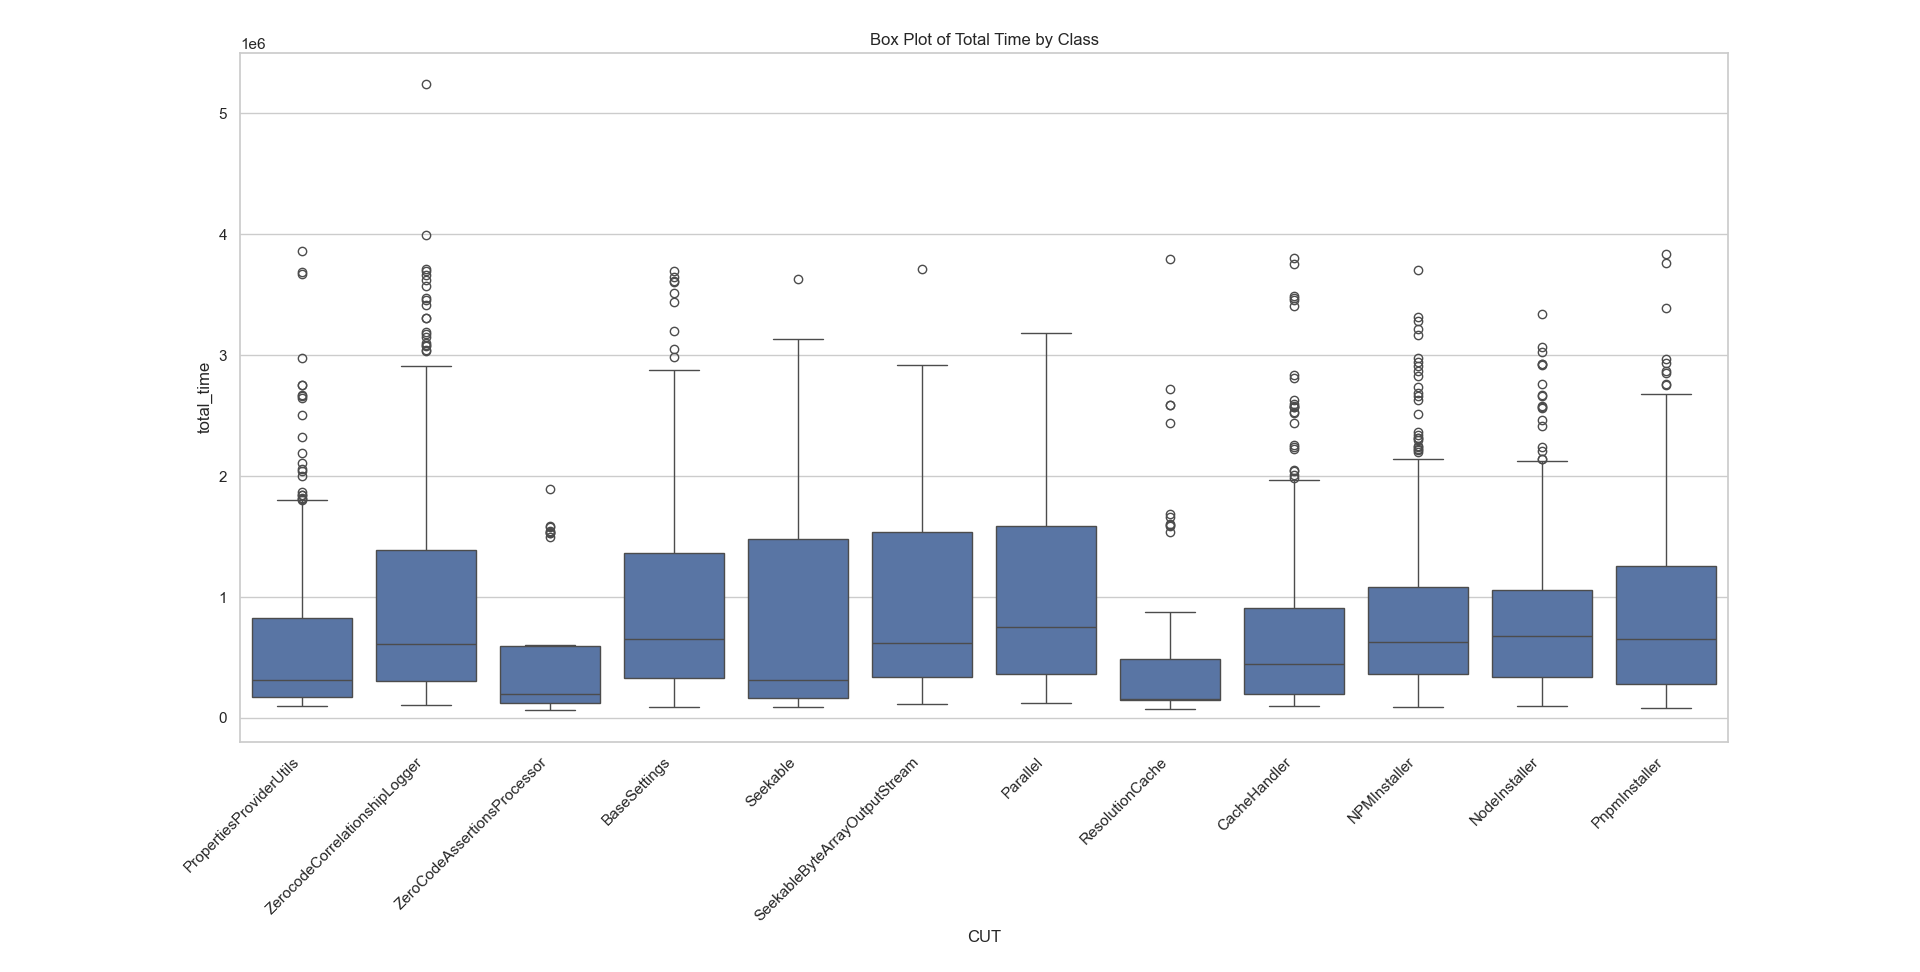
\includegraphics[width=1\textwidth]{images/total_time_by_class.png}
\caption{Total time taken by each class}
\label{fig:time_class}
\end{figure}

\begin{figure}[H]
\centering
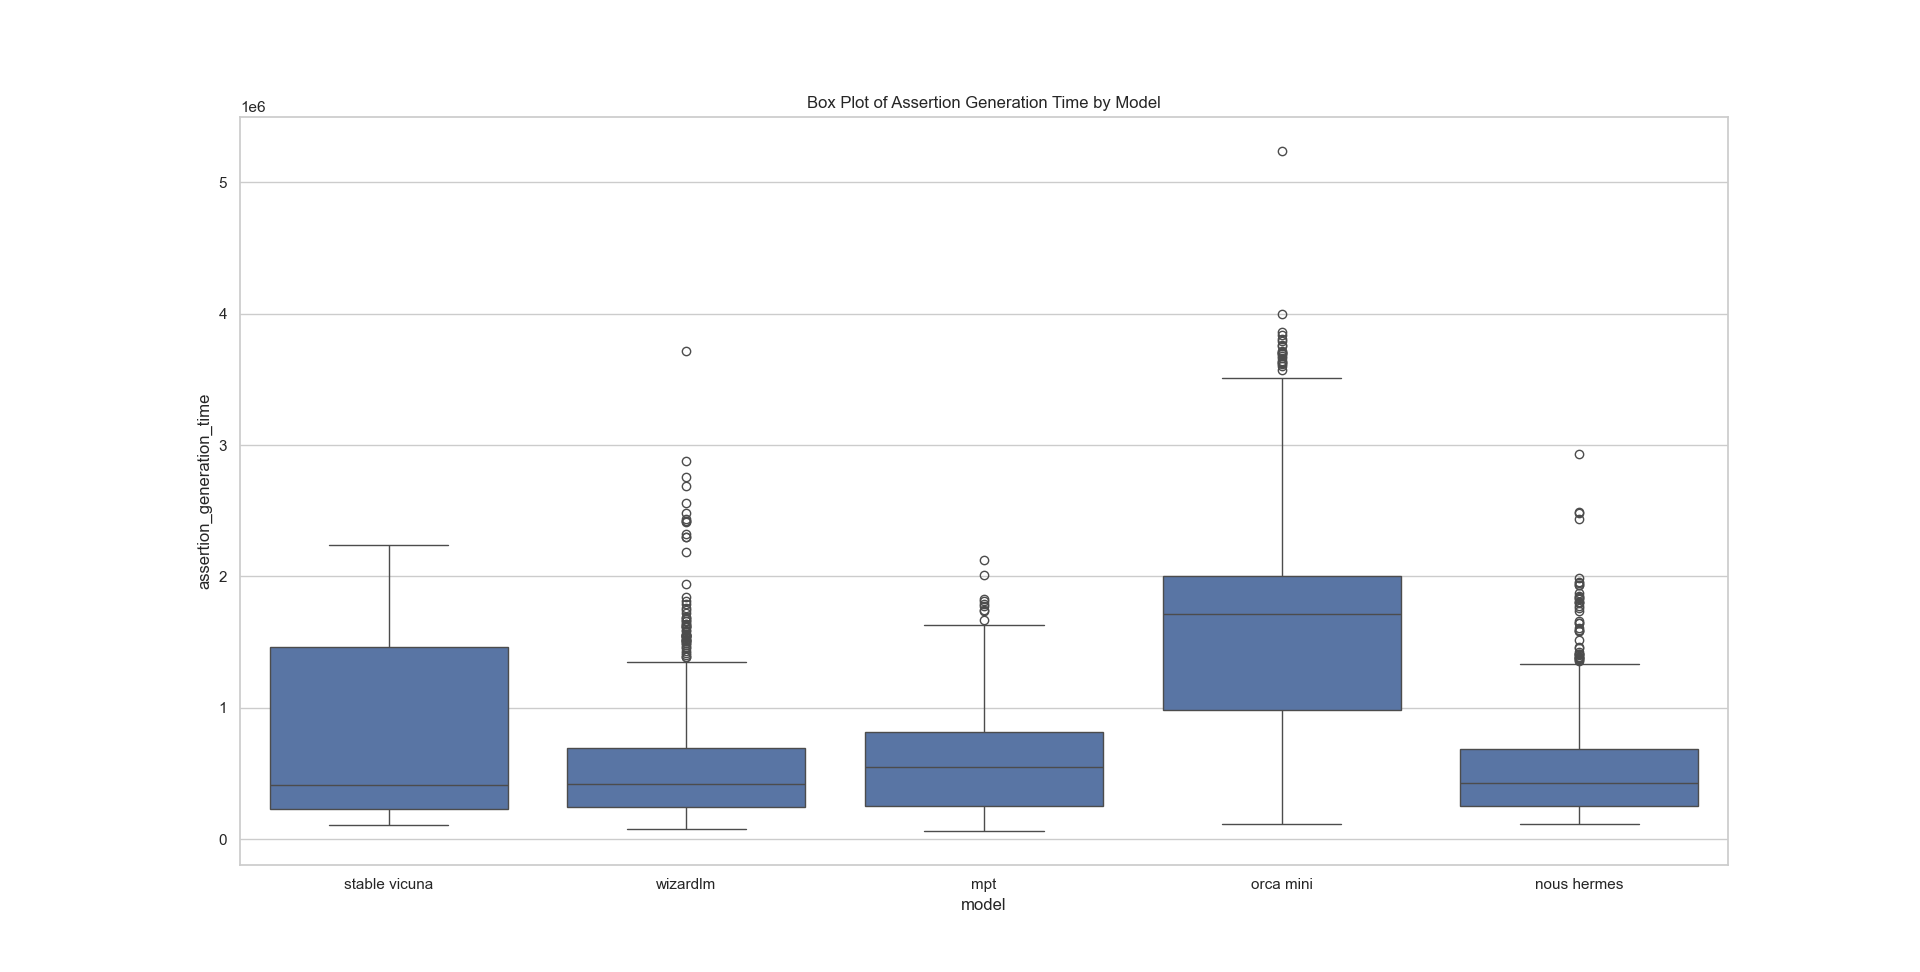
\includegraphics[width=1\textwidth]{images/assertion_time_by_model.png}
\caption{Assertion generation time taken by each model}
\label{fig:assertion_time_models}
\end{figure}

\begin{figure}[H]
\centering
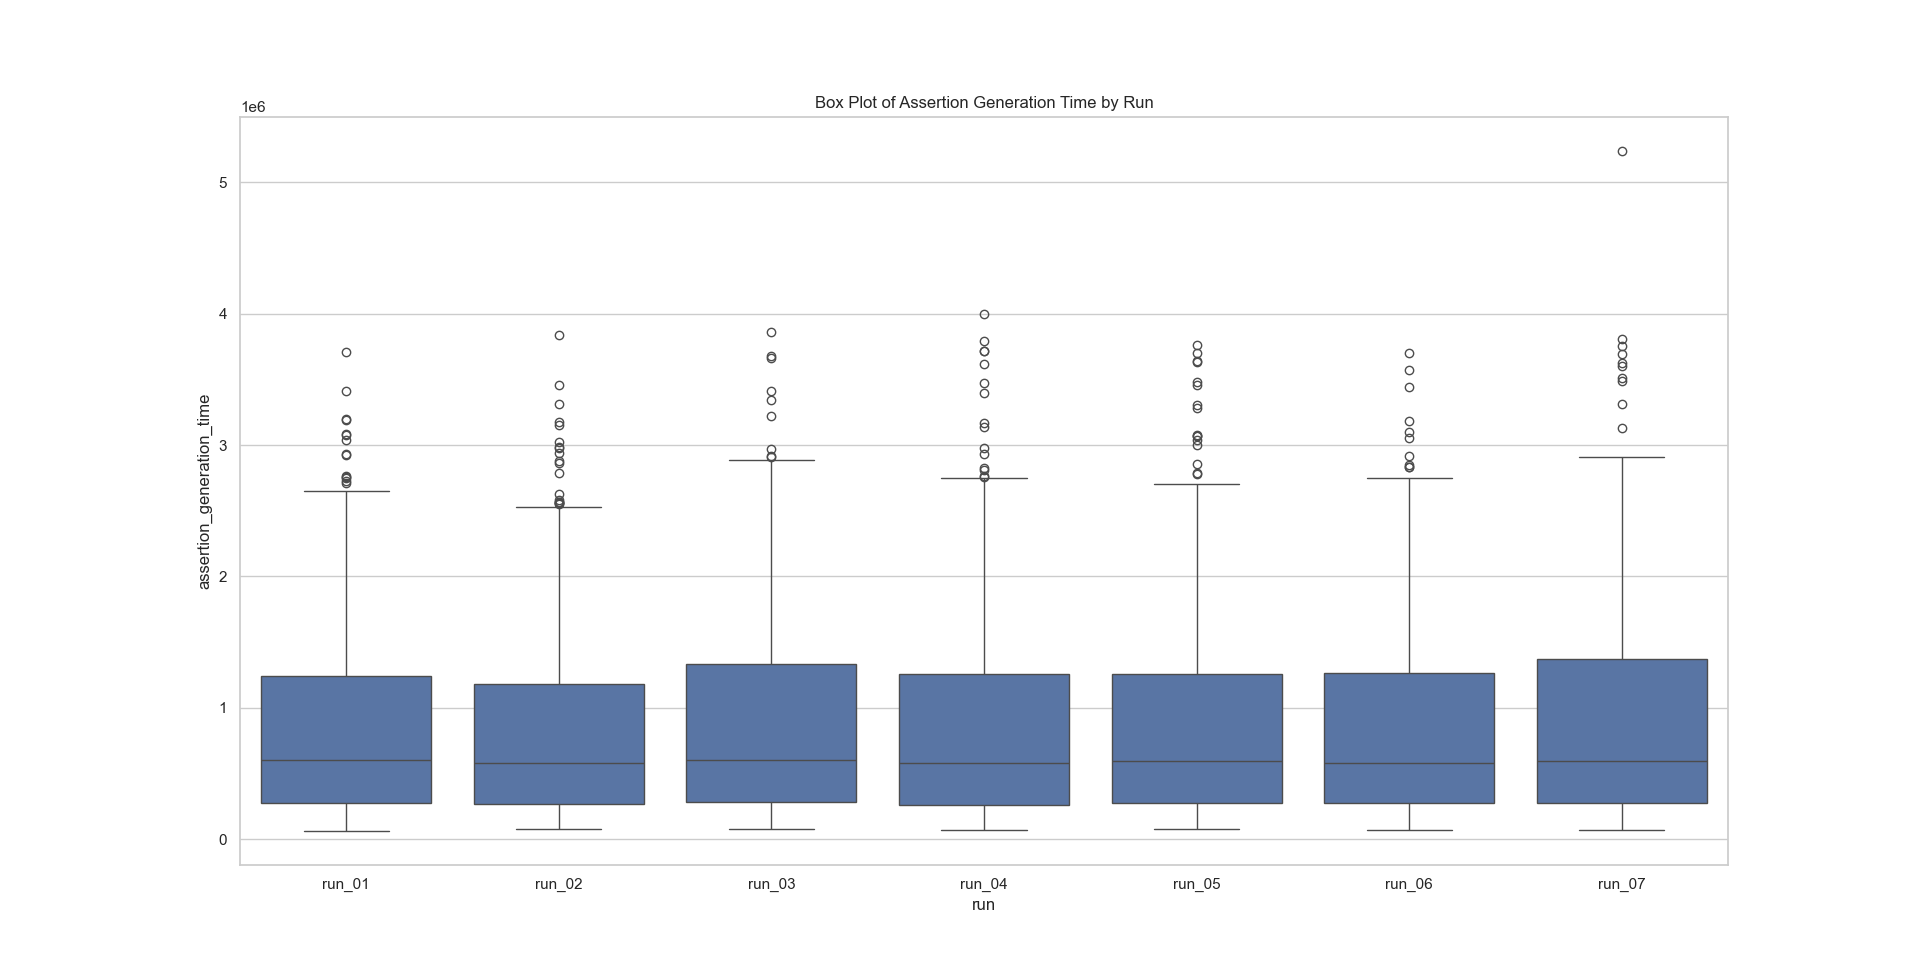
\includegraphics[width=1\textwidth]{images/assertion_time_by_runs.png}
\caption{Assertion generation time taken by each run}
\label{fig:assertion_time_runs}
\end{figure}

\begin{figure}[H]
\centering
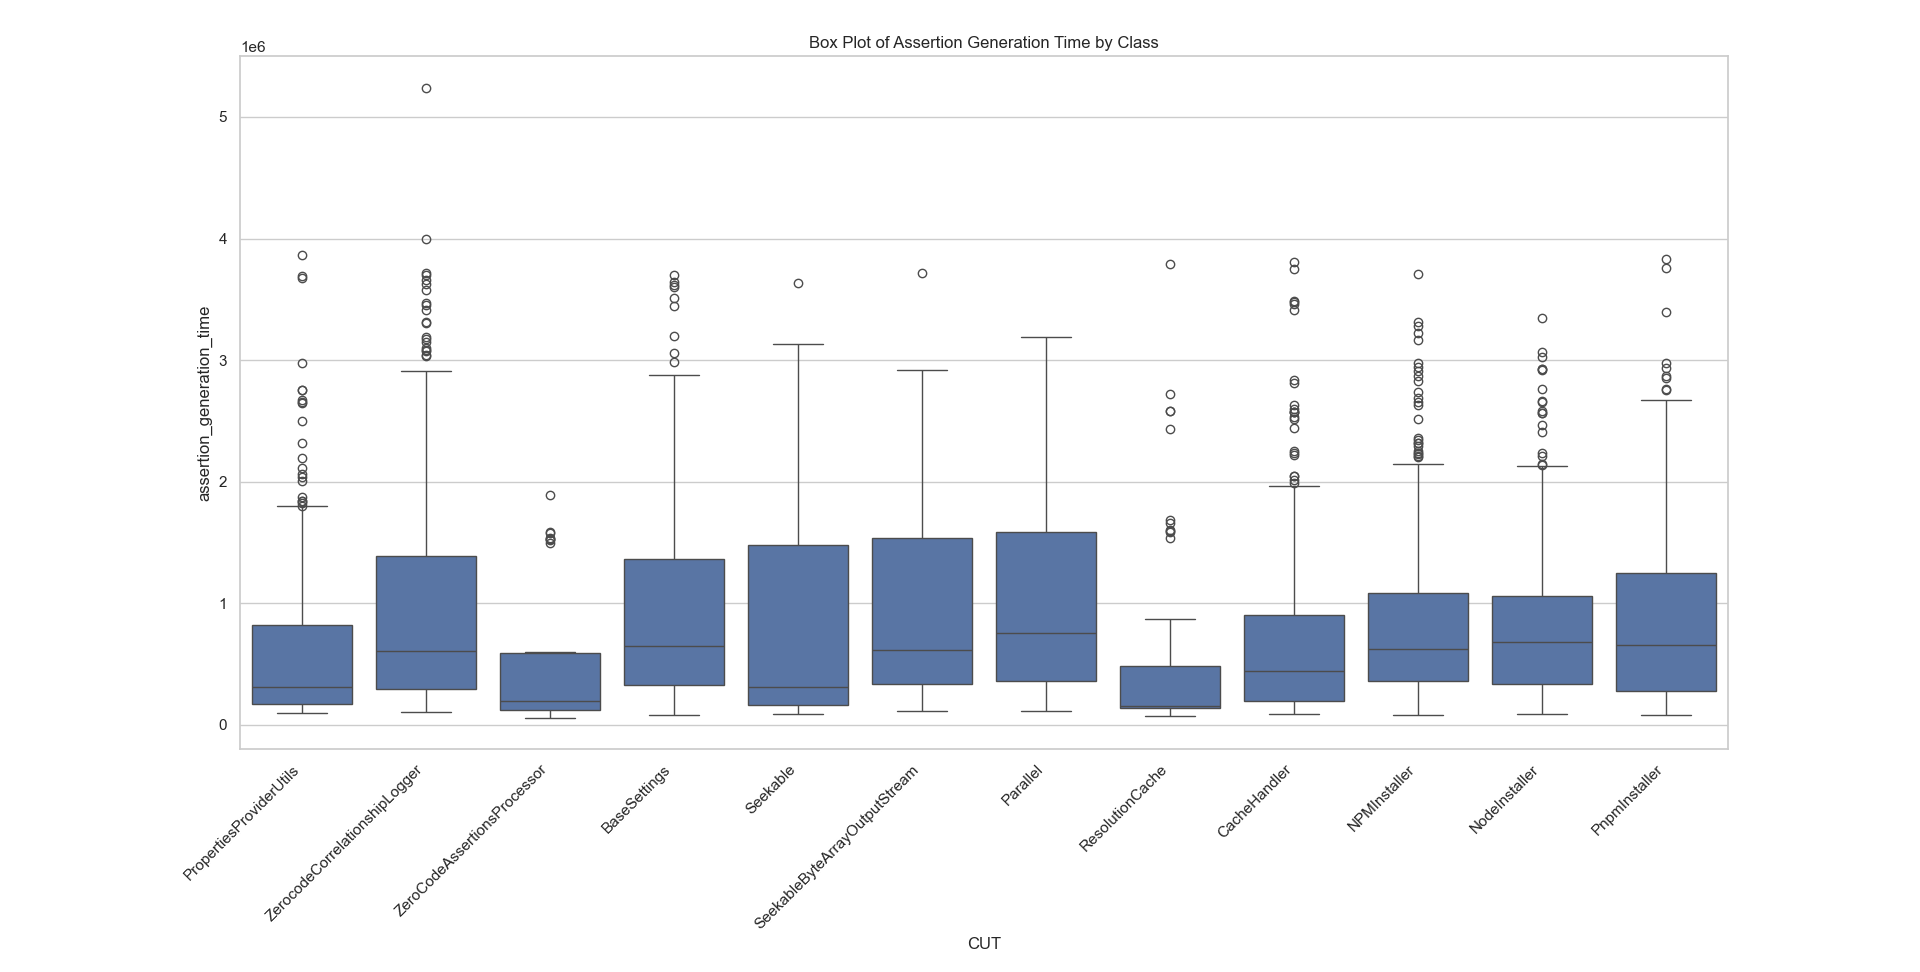
\includegraphics[width=1\textwidth]{images/assertion_time_by_class.png}
\caption{Assertion generation time taken by each class}
\label{fig:assertion_time_class}
\end{figure}

\vspace{0.1 cm}
\subsection{RQ2}
\label{sec:results_rq2}
\vspace{0.1 cm}

In this subsection, an overview of ...

\section{Threats to Validity}
\label{sec:t2v}
\vspace{0.2 cm}

The study acknowledges several potential threats to its validity.

\begin{enumerate}
    \item \textbf{Randomness in LLM Outputs:} One significant threat to the study's validity stems from the inherent randomness associated with Large Language Models (LLMs). The generated outputs are subject to variations based on the model's training conditions and prompt inputs, potentially impacting the reproducibility and consistency of results. In order to minimize the variation, we ran each experiments 7 times and took the median results.

    \item \textbf{Generalizability to Diverse Datasets:} The study recognizes the potential limitation of generalizability to other datasets or programming languages. The findings, rooted in the analysis of Java projects from GitHub, may not extend seamlessly to different programming communities or languages, highlighting a domain-specific consideration.

    \item \textbf{Dataset-Induced Bias:} The dataset itself, composed of Java projects sourced from GitHub, introduces a possible bias reflective of the practices and characteristics specific to the Java programming community on this platform. This inherent bias could influence the study's conclusions and their applicability to broader software development contexts.

    \item \textbf{Concerns of Data Leakage:} In addressing concerns related to data leakage, the study takes precautionary measures by excluding candidate repositories that might appear in the pretraining corpus of the LLMs. This step aims to ensure the integrity of the evaluation process and prevent inadvertent leakage of information.

    \item \textbf{Selection Bias from Compilation and Execution Requirements:} The imposition of specific compilation and execution requirements, such as using Maven as the package manager and ensuring compatibility, introduces a potential source of selection bias. The study acknowledges the impact of these criteria on the composition of the chosen repositories, potentially affecting the representativeness of the dataset.

    \item \textbf{Evaluation Metrics Limitations:} The study recognizes the limitations of the chosen evaluation metrics and criteria. While these metrics provide a quantitative basis for assessment, they may not comprehensively capture the nuanced aspects of LLM-based test oracle generation. This acknowledgment indicates a need for a holistic understanding beyond the quantitative measures employed.
\end{enumerate}

These considerations collectively contribute to the study's robustness and transparency, providing insights into potential factors that may influence the interpretation and application of its findings.

\section{Discussion}
\label{sec:discussion}
\vspace{0.2 cm}

Diving into a comprehensive discussion of our experiments and findings unveils nuanced insights into the intricate landscape of automated testing practices, particularly in the context of leveraging Large Language Models (LLMs) for test oracle generation. The empirical analysis of our approach to generating oracles for unit test cases provides a nuanced understanding of the challenges and potential breakthroughs in this domain. As we navigate the landscape of automated testing, it becomes evident that the multifaceted nature of test cases poses unique challenges that demand innovative solutions.

The comparative analysis between LLM-generated assertions and traditional automated test generation tools, exemplified by EvoSuite, brings to light unexpected and valuable results. The effectiveness and efficiency of LLM-based approaches did not universally outperform traditional methods, marking a noteworthy observation that prompts a deeper exploration into the factors influencing assertion quality and the overall testing workflow.

Surprisingly, LLMs, despite their profound capabilities in understanding natural language, grapple with the complexity of translating this understanding into precise code-related tasks. This observation raises critical questions about the adaptability of LLMs to the diverse nature of test cases, each with its unique intricacies and requirements for meaningful assertions. As developers interact with LLM-generated assertions, a spectrum of sentiments emerges, reflecting the potential and challenges in incorporating advanced language models into the day-to-day software development processes.

Moreover, the results of Research Question 2, indicating an average time of 8.24 minutes for assertion generation for a single test case, shed light on a usability challenge. This prompts considerations about real-world practicality, prompting us to explore alternative approaches, including leveraging APIs like ChatGPT\cite{chatgpt}, Bard\cite{bard}, GooseAI\cite{gooseai}, Cohere\cite{cohere}, Claude\cite{claude}, LLaMA\cite{LLaMA}, PaLM\cite{palm} for faster and potentially more efficient interactions.

It's important to highlight that the models utilized in our experiments are general-purpose Large Language Models\cite{}, not specifically fine-tuned for code generation like Codex\cite{finnie-ansley_robots_2022}. Consequently, precise and thoughtful prompting is crucial when engaging with these models. Since they lack specialized training for code-related tasks, providing clear and context-rich instructions becomes paramount to ensure accurate and relevant responses. This characteristic underscores the need for developers to be mindful of the model's general nature and adapt their prompts accordingly for optimal results in the context of code-related inquiries.